\clearpage % Ends the current page and causes all figures and tables to be printed
\begin{figure*}[p] % The * makes the figure span both columns, p places the figure on a float page
  \begin{center}
 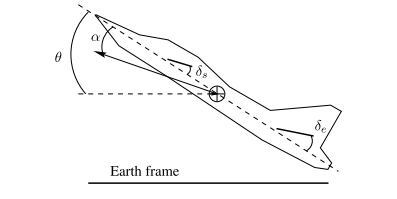
\includegraphics[width=0.7\textwidth]{images/problem/aircraft.png}
  \end{center}
  \caption{Aircraft model considered, obtained from ~\cite[p. 15]{Exercises:2015}.}
  \label{fig:aircraft}
\end{figure*}
\begin{figure*}[p] % The * makes the figure span both columns, p places the figure on a float page
  \begin{center}
 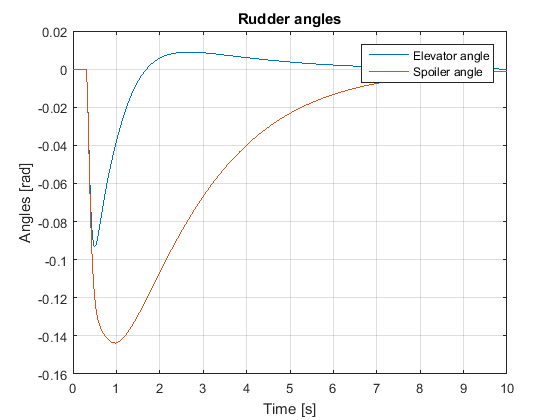
\includegraphics[width=0.8\textwidth]{images/sol2/rudderangles1.png}
  \end{center}
  \caption{Plot of the rudder angles by simulating the system using the PD-Controller as model for the pilot and \emph{design1} settings.}
  \label{fig:rangles1}
\end{figure*}

\begin{figure*}[p] % The * makes the figure span both columns, p places the figure on a float page
  \begin{center}
 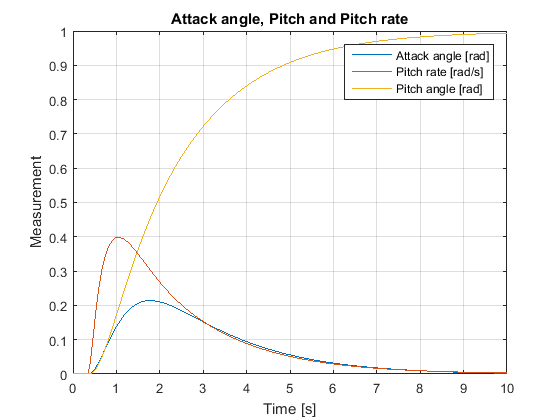
\includegraphics[width=0.8\textwidth]{images/sol2/rudderangles2.png}
  \end{center}
  \caption{Plot of the angle of attack, pitch and pitch rate by simulating the system using the PD-Controller as model for the pilot and \emph{design1} settings.}
  \label{fig:rangles2}
\end{figure*}

%solution 3
\begin{figure*}[p] % The * makes the figure span both columns, p places the figure on a float page
  \begin{center}
 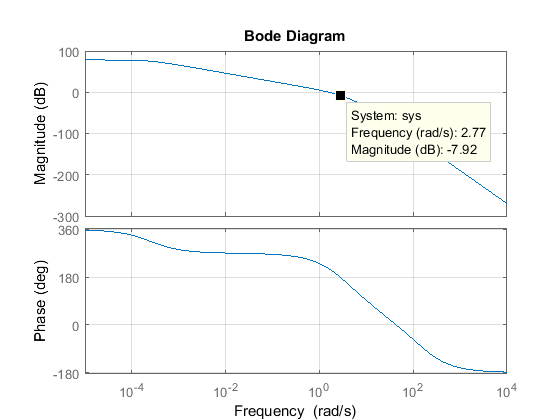
\includegraphics[width=0.8\textwidth]{images/sol3/bodeol2.png}
  \end{center}
  \caption{Bode plot of the linearised open loop using the relay model for the pilot and \emph{design1} settings.}
  \label{fig:sim2bode}
\end{figure*}

\begin{figure*}[p] % The * makes the figure span both columns, p places the figure on a float page
  \begin{center}
 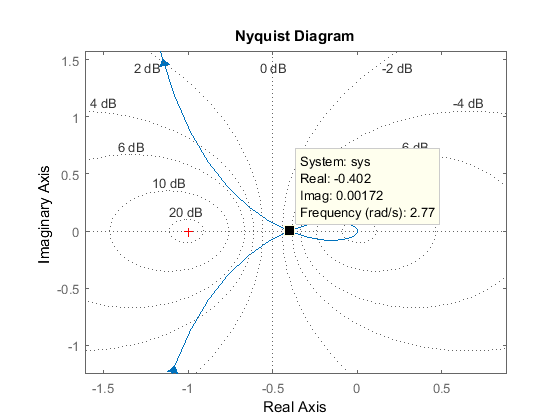
\includegraphics[width=0.8\textwidth]{images/sol3/nyquist2.png}
  \end{center}
  \caption{Nyquist plot of the linearised open loop using the relay model for the pilot and \emph{design1} settings.}
  \label{fig:sim2nyquist}
\end{figure*}

% \begin{figure*}[p] % The * makes the figure span both columns, p places the figure on a float page
%   \begin{center}
%  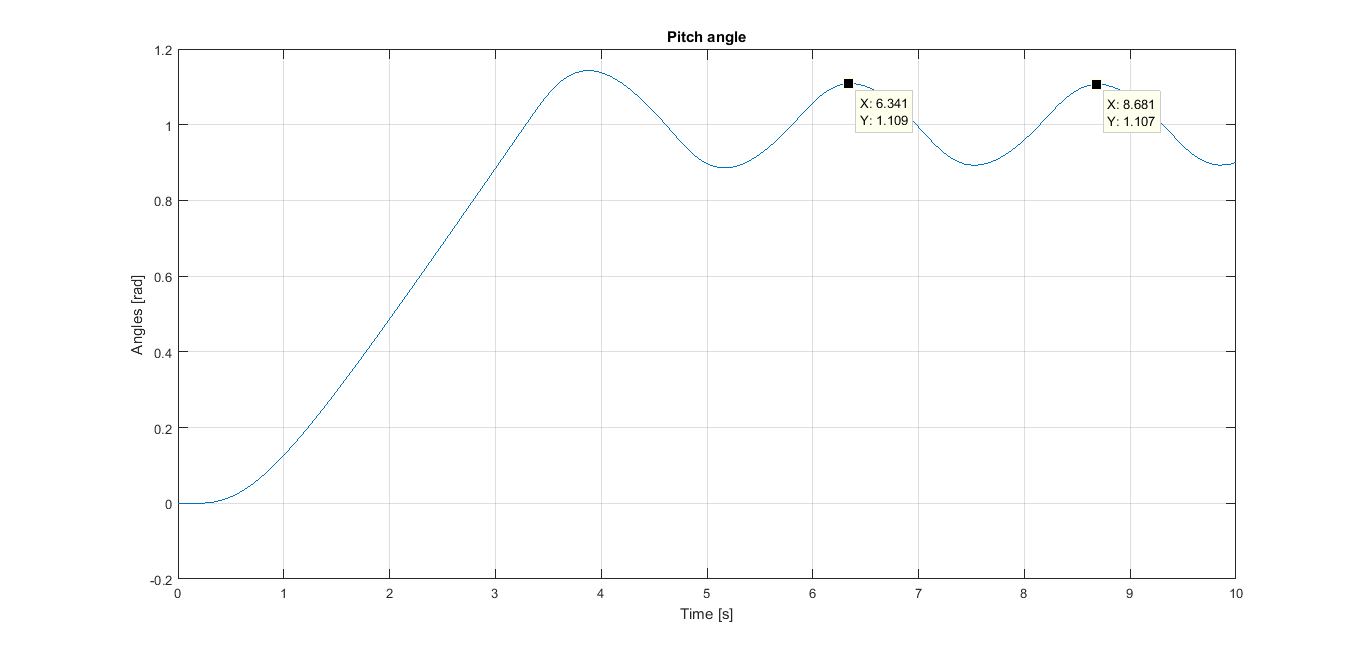
\includegraphics[width=0.8\textwidth]{images/sol3/oscillations.png}
%   \end{center}
%   \caption{Plot of the pitch angle by simulating the system using the relay  model for the pilot and \emph{design1} settings.}
%   \label{fig:sim2pitch}
% \end{figure*}

%solution 4
\begin{figure*}[p] % The * makes the figure span both columns, p places the figure on a float page
  \begin{center}
 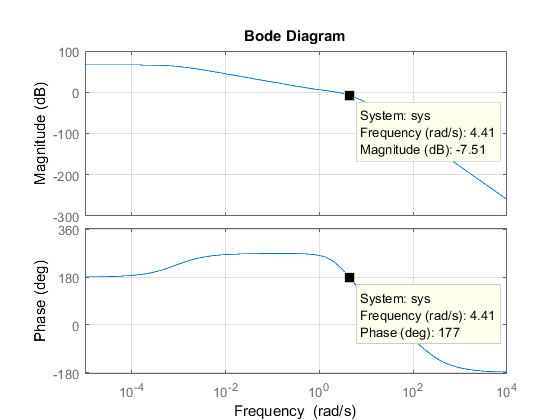
\includegraphics[width=0.8\textwidth]{images/sol4/bodeplot2.png}
  \end{center}
  \caption{Bode plot of the linearised open loop using the relay model for the pilot and \emph{design2} settings.}
  \label{fig:bode2}
\end{figure*}

\begin{figure*}[p] % The * makes the figure span both columns, p places the figure on a float page
  \begin{center}
 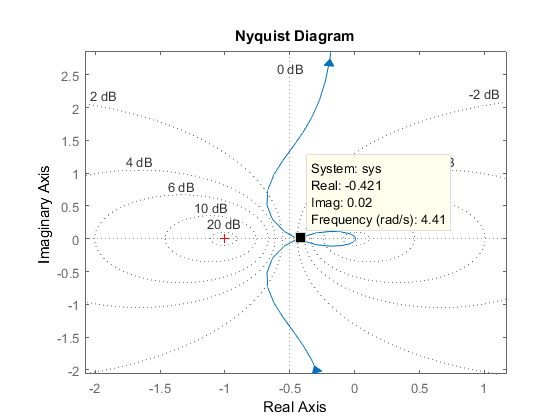
\includegraphics[width=0.8\textwidth]{images/sol4/nyquist2.png}
  \end{center}
  \caption{Nyquist plot of the linearised open loop using the relay model for the pilot and \emph{design2} settings.}
  \label{fig:nyquist2}
\end{figure*}
\begin{figure*}[p] % The * makes the figure span both columns, p places the figure on a float page
  \begin{center}
 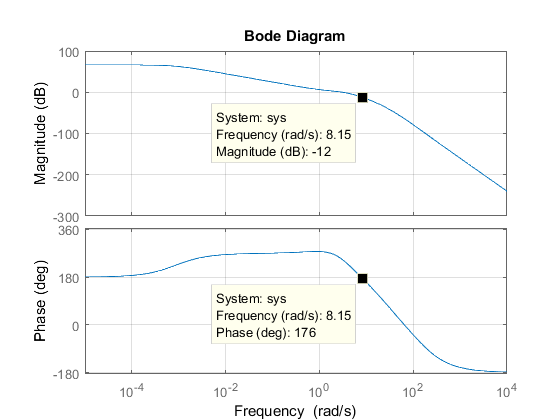
\includegraphics[width=0.8\textwidth]{images/sol4/bodeplot3.png}
  \end{center}
  \caption{Bode plot of the linearised open loop using the relay model for the pilot and \emph{design3} settings.}
  \label{fig:bode3}
\end{figure*}

\begin{figure*}[p] % The * makes the figure span both columns, p places the figure on a float page
  \begin{center}
 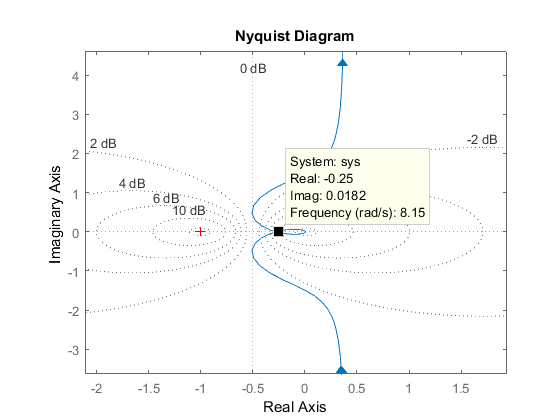
\includegraphics[width=0.8\textwidth]{images/sol4/nyquist3.png}
  \end{center}
  \caption{Nyquist plot of the linearised open loop using the relay model for the pilot and \emph{design3} settings.}
  \label{fig:nyquist3}
\end{figure*}

\begin{figure*}[p] % The * makes the figure span both columns, p places the figure on a float page
  \begin{center}
 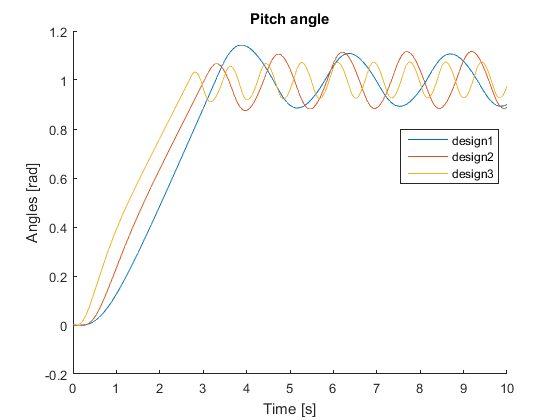
\includegraphics[width=0.8\textwidth]{images/sol4/comparative.png}
  \end{center}
  \caption{Plots of the pitch angle by simulating the system using the relay model for the pilot and \emph{design1}, \emph{design2} and \emph{design3} settings.}
  \label{fig:comparative}
\end{figure*}

%solution5
\begin{figure*}[p] % The * makes the figure span both columns, p places the figure on a float page
  \begin{center}
 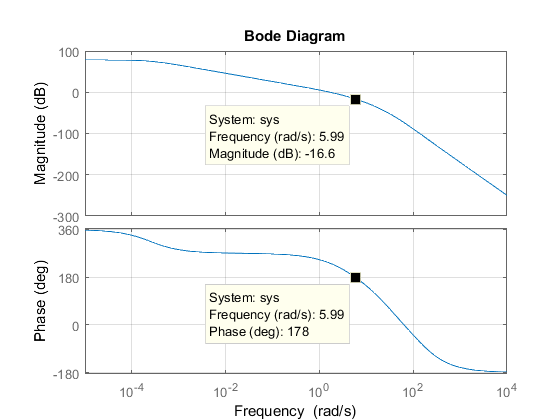
\includegraphics[width=0.8\textwidth]{images/sol5/bodeimp.png}
  \end{center}
  \caption{Bode plot of the linearised open loop using the relay model for the pilot and suggested design.}
  \label{fig:bodeimp}
\end{figure*}

\begin{figure*}[p] % The * makes the figure span both columns, p places the figure on a float page
  \begin{center}
 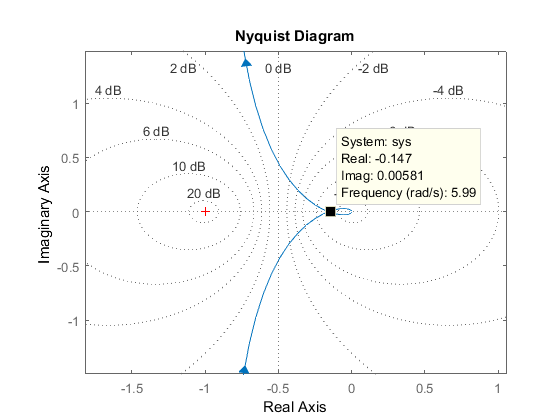
\includegraphics[width=0.8\textwidth]{images/sol5/nyquistimp.png}
  \end{center}
  \caption{Nyquist plot of the linearised open loop using the relay model for the pilot suggested design.}
  \label{fig:nyquistimp}
\end{figure*}
\begin{figure*}[p] % The * makes the figure span both columns, p places the figure on a float page
  \begin{center}
 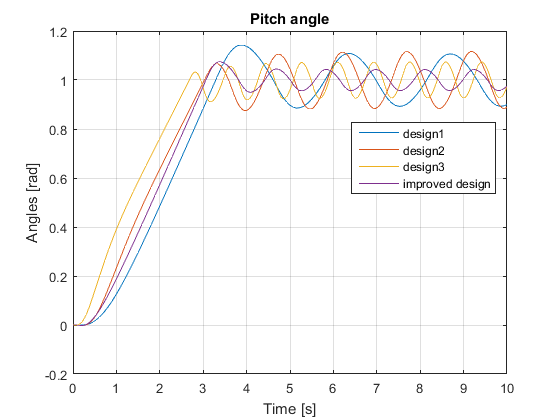
\includegraphics[width=0.8\textwidth]{images/sol5/improved.png}
  \end{center}
  \caption{Plots of the pitch angle by simulating the system using the relay model for the pilot and \emph{design1}, \emph{design2} and \emph{design3} settings, comparing them to the improved design suggested in question \textbf{5}.}
  \label{fig:improved}
\end{figure*}

%solution6

\begin{figure*}[p] % The * makes the figure span both columns, p places the figure on a float page
  \begin{center}
 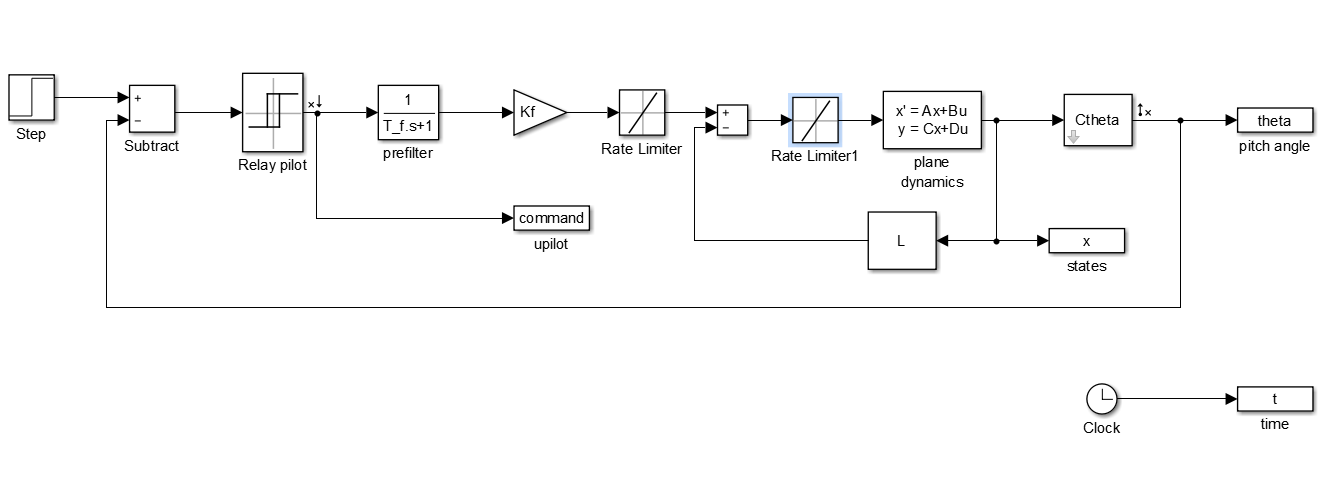
\includegraphics[width=\textwidth]{images/sol6/figcircuit.png}
  \end{center}
  \caption{Simulink model of the aircraft including the rate limiters applied on both the pilot command and on the sum of the pilot command and feedback command.}
  \label{fig:sol6circuit}
\end{figure*}


\begin{figure*}[p] % The * makes the figure span both columns, p places the figure on a float page
  \begin{center}
 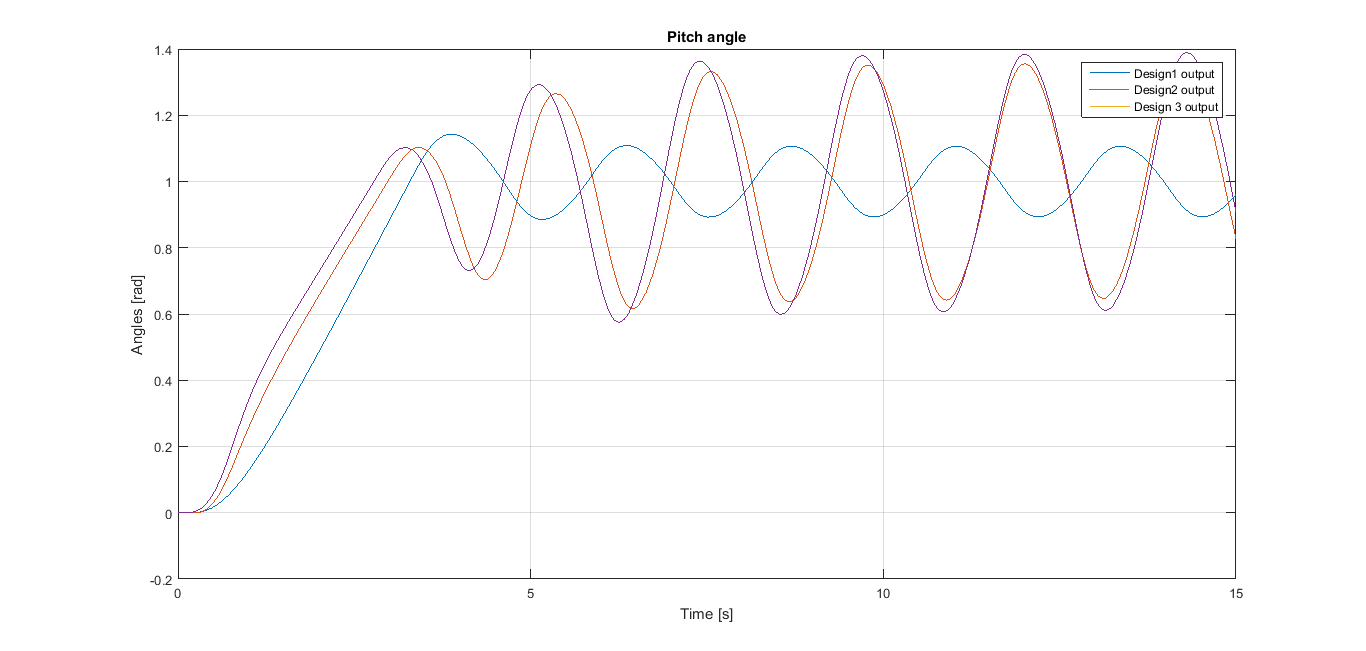
\includegraphics[width=0.8\textwidth]{images/sol6/fig1lowlimit.png}
  \end{center}
  \caption{Pitch angle plot for the various design using a rate limit $r=0.5$.}
  \label{fig:sol6lowlimit}
\end{figure*}

\begin{figure*}[p] % The * makes the figure span both columns, p places the figure on a float page
  \begin{center}
 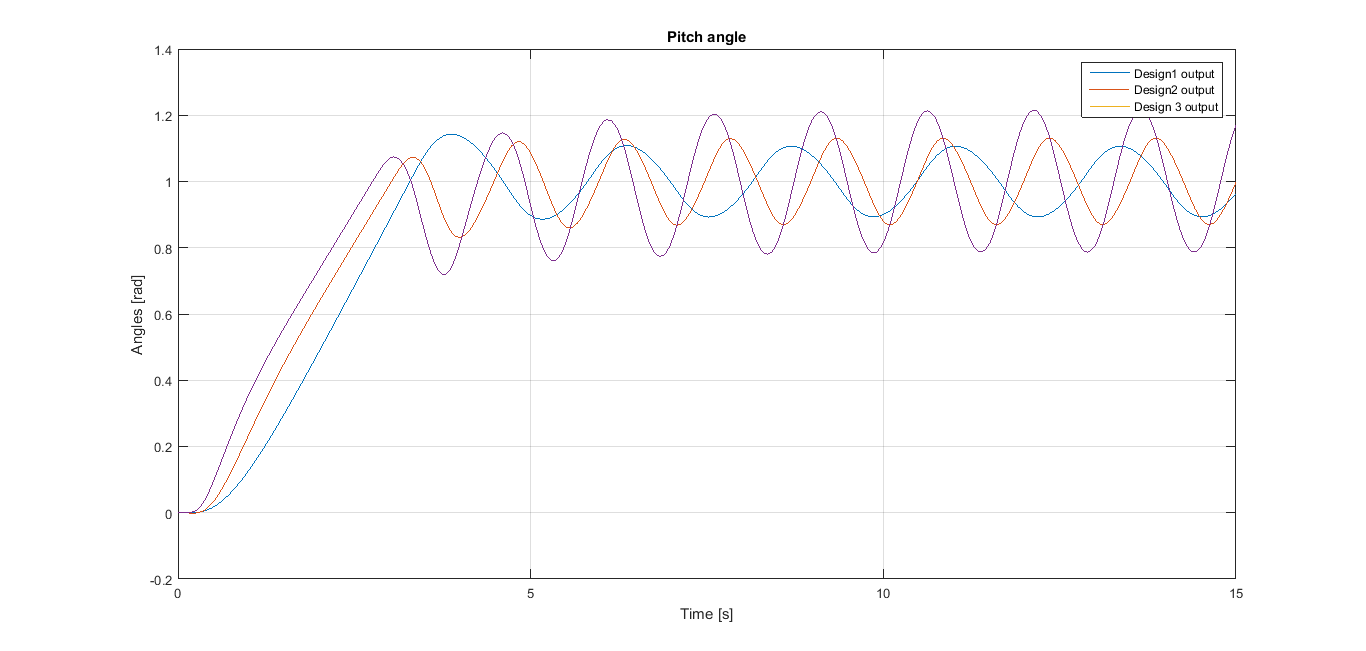
\includegraphics[width=0.8\textwidth]{images/sol6/fig2highlimit.png}
  \end{center}
  \caption{Pitch angle plot for the various design using a rate limit $r=1$.}
  \label{fig:sol6highlimit}
\end{figure*}


\begin{figure*}[p] % The * makes the figure span both columns, p places the figure on a float page
  \begin{center}
 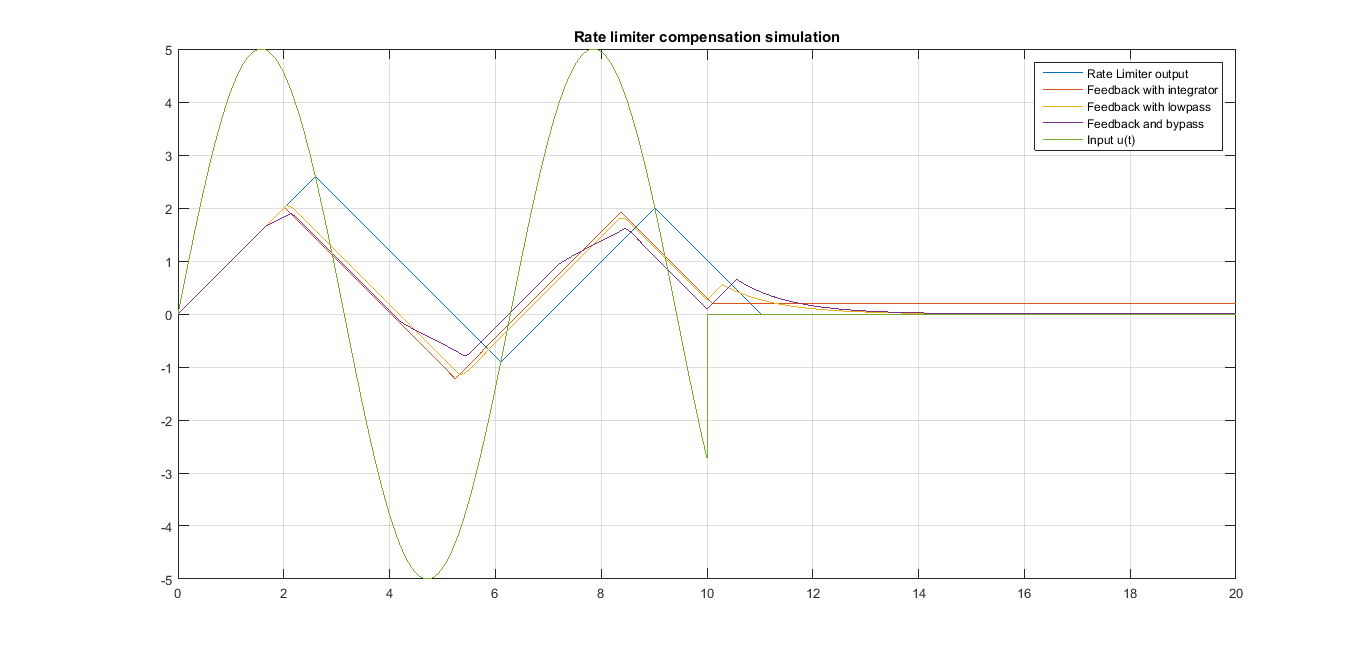
\includegraphics[width=0.8\textwidth]{images/sol6/simulationfilters.png}
  \end{center}
  \caption{Simulation of the various rate limiter filters for an input signal $u(t)=5\sin(t)$ for $t \leq 10$, $u(t)=0$ for $t > 10$. The rate limiters have rate limit value $r=1$.}
  \label{fig:simfilters}
\end{figure*}
\begin{figure*}[p] % The * makes the figure span both columns, p places the figure on a float page
  \begin{center}
 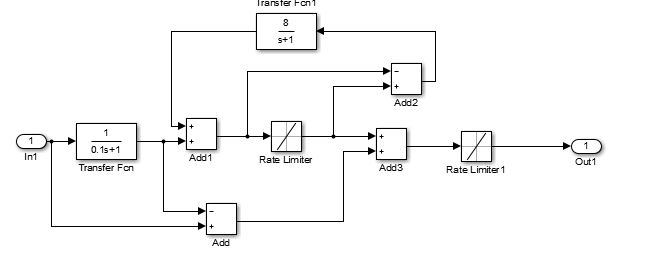
\includegraphics[width=0.8\textwidth]{images/sol6/filter.png}
  \end{center}
  \caption{Rate limiter filter with feedback and bypass [3].}
  \label{fig:filter}
\end{figure*}